\documentclass{beamer}

\usepackage{amsmath}

%\usetheme{}

\mode<presentation>

%Information to be included in the title page:
\title{Comparing Classical and Nonclassical Symmetries of Nonlinear Partial Differential Equations}
\author{William Helman and Daniel Sinderson}
\institute{Southern Oregon University}
\date{2023}

\begin{document}

\frame{\titlepage}
\begin{frame}
    \frametitle{Table of Contents}
    \tableofcontents
\end{frame}

\section{Introduction}
    \subsection{Project Goal}
    \subsection{What is a Symmetry?}
    \subsection{What is a Differential Equation?}
    \subsection{Background on our Equations}
\section{Results}
    \subsection{Classical Symmetries}
    \subsection{Nonclassical Symmetries}
\section{Conclusion}
    \subsection{Discussion}
    \subsection{Open Questions}
    \subsection{Next Steps}



\begin{frame}
    \frametitle{Project Goal}
    Our research objective for this project was to calculate the classical and nonclassical symmetry groups for the reduced Gibbons-Tsarev equation and the Born-Infeld equation and compare them.
\end{frame}



\begin{frame}
    \frametitle{What is a Symmetry?}
    \begin{definition}<1->
        A symmetry is a transformation that leaves an object invariant.
    \end{definition}
    \vspace*{0.5in}
    \begin{definition}<2->
        A symmetry is a change that doesn't change anything.
    \end{definition}
\end{frame}


\begin{frame}
    \frametitle{What is a Symmetry?}
    Let's see this in action using the simple linear equation $x-y=0$.\\
    \begin{center}
        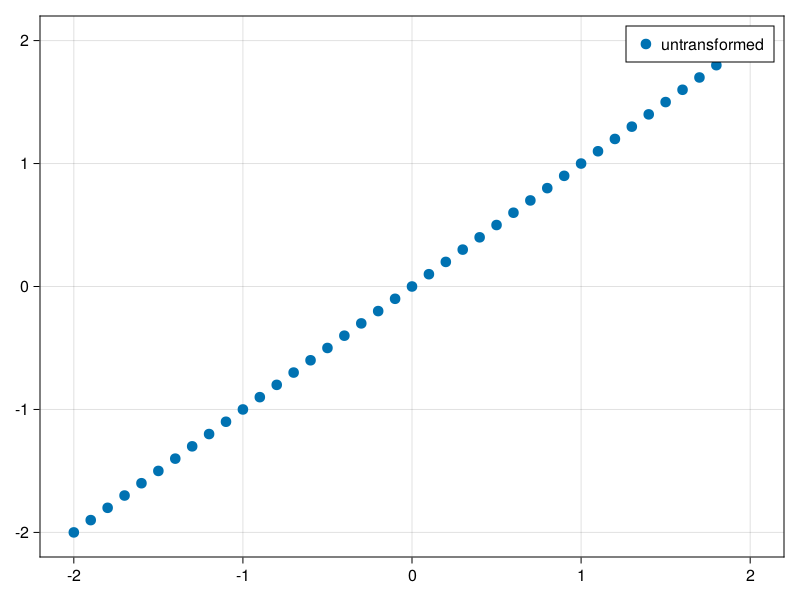
\includegraphics[width=9cm]{y=x.png}
    \end{center}
\end{frame}

\begin{frame}
    \frametitle{What is a Symmetry?}
    \begin{example}[A Non-Example]
        \begin{itemize}
            \item For our first transformation, let's define new variables\\ $\bar{x}=x+1$ and $\bar{y}=y$.
            \item Now we rewrite our equation using these new variables. \begin{equation*}
                \begin{aligned}
                    \bar{x}-\bar{y} &= 0 & \text{by definition} \\
                    x+1-y &= 0 & \text{by substitution} \\
                    y &= x+1 & \text{by rewriting in slope-intercept form}
                \end{aligned}
            \end{equation*}
            \item This transformation is not a symmetry: \\ $x-y+1\ne x-y$
        \end{itemize}        
    \end{example}
\end{frame}


\begin{frame}
    \frametitle{What is a Symmetry?}
    \framesubtitle{A Transformation that is a Symmetry}
    \begin{example}[2]<1->
        \begin{itemize}
            \item Let's define some new variables again\\ $\bar{x}=x+1$ and $\bar{y}=y+1$.
            \item Now we rewrite our equation using these new variables. \begin{equation*}
                \begin{aligned}
                    \bar{x}-\bar{y} &= 0 & \text{by definition} \\
                    (x+1)-(y+1) &= 0 & \text{by substitution} \\
                    (x-y)+(1-1) &= 0 & \text{by algebra} \\
                    x-y &= 0 & \text{by algebra} \\
                    y &= x & \text{by rewriting in slope-intercept form}
                \end{aligned}
            \end{equation*}
            \item This transformation is a symmetry: \\ $x-y = x-y$
        \end{itemize}        
    \end{example}
\end{frame}


\begin{frame}
    \frametitle{What is a Symmetry?}
    The graphs of our three equations.\\
    \begin{center}
        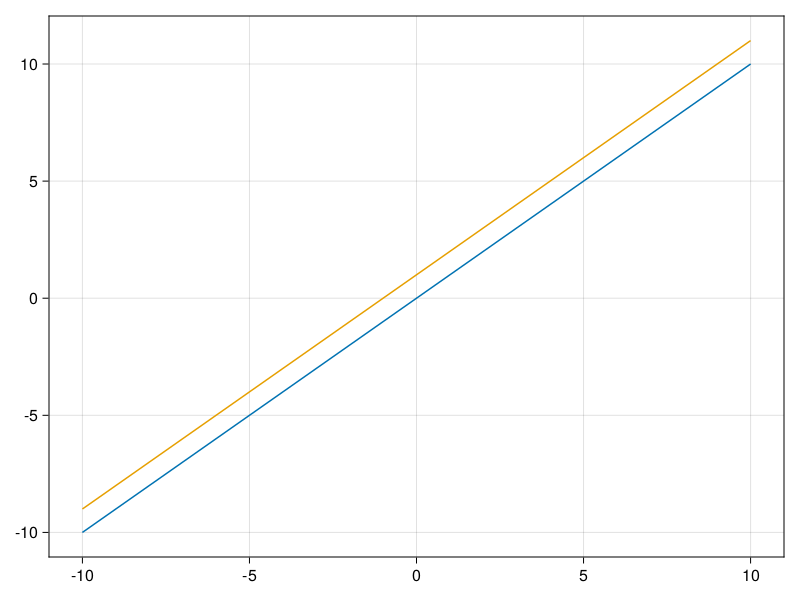
\includegraphics[width=9cm]{y=x+1.png}
    \end{center}
\end{frame}



\begin{frame}
    \frametitle{What is a Symmetry?}
    \begin{Large}
        Who cares?
    \end{Large}
    \vspace*{0.25in}
    \begin{itemize}
        \item Symmetries help us understand and solve equations that we wouldn't normally be able to.\pause
        \item Symmetries encode physically meaningful aspects of equations, like conservation laws in physics.\pause
    \end{itemize}
\end{frame}



\begin{frame}
    \frametitle{What is a Differential Equation?}
    \begin{definition}
    \begin{itemize}
        \item A differential equation is an equation that contains both an unknown function and information about how that function relates to its rates of change. \pause
        \item Differential equations show up everywhere we model something using information about how that thing changes over time. This includes everything from population dynamics to the motion of the planets. \pause
        \item Differential equations are different from algebraic equations, and can't be solved in the same ways.
    \end{itemize}
\end{definition}
\end{frame}



\begin{frame}
    \frametitle{What is a Differential Equation?}
    As an example, we'll use the equation for an undamped spring.\\
    \vspace*{0.125in}
    \begin{Large}
        $$m\ddot{x}=-\kappa{x}$$
    \end{Large}
    \vspace*{0.25in}
    \begin{itemize}
        \item Here $m$ is the mass, $\ddot{x}$ is the acceleration, $\kappa$ is the spring constant, and $x$ is the position.
        \item If we set both $m$ and $\kappa$ to $1$, we get $\ddot{x}=-x$.
        \item This is a simple differential equation with the algebraic solution of $x(t)=c_1\cos(t)+c_2\sin(t)$.
    \end{itemize}
\end{frame}


\begin{frame}
    \frametitle{What is a Differential Equation?}
    The graph of our spring system $x(t)=\cos(t)+\sin(t)$, where $c_1=c_2=1$.\\
    \begin{center}
        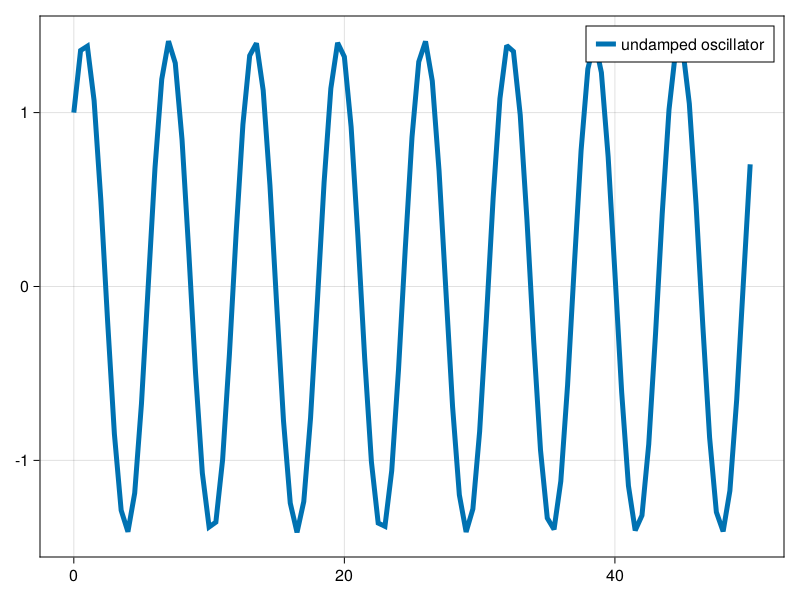
\includegraphics[width=9cm]{undamped.png}
    \end{center}
\end{frame}


\begin{frame}
    \frametitle{The History of the Born-Infeld and the reduced Gibbons-Tsarev Equations}

\end{frame}



\begin{frame}
    \frametitle{The Classical Symmetries of the Born-Infeld and the reduced Gibbons-Tsarev Equations}
    \begin{itemize}
        \item To find the classical symmetries for a differential equation, you have to solve for Lie's Invariance Condition.
        \item Lie's Invariance Condition changes based on the type and order of differential equation.
        \item For second order partial differential equations like we had, Lie's Invariance condition is as follows
    \end{itemize}
    \begin{Large}
        $$\Gamma^{2}(\Delta)$$
    \end{Large}
\end{frame}



\begin{frame}
    \frametitle{The Nonclassical Symmetries of the Born-Infeld and the reduced Gibbons-Tsarev Equations}

\end{frame}



\begin{frame}
    \frametitle{Future Work: Does Integrability Imply Equivalence of Classical and Nonclassical Symmetries?}

\end{frame}



\begin{frame}
    \frametitle{Future Work: Does Equivalence of Classical and Nonclassical Symmetries Imply Integrability?}

\end{frame}



\end{document}